\documentclass[a4paper, 12pt]{scrbook}
%%%------------------%%%
%%%  load the design %%%
%%%------------------%%%
%%%%% ------------------------------------------------%%%%%
%%%%% graphic engine
%%%%% ------------------------------------------------%%%%%
%% Dual Mode
%%
%% Put the pic in the './images' folder. Use the Makefile
%% to convert the images to eps and pdf files. Then
%% the needed pic are selected automaticly by the
%% selected engine (pdf or eps)
%%
\usepackage{graphicx}
\graphicspath{{images_pdf/},{images_eps/}}
%\usepackage{chicago}
\usepackage{amsmath}
\usepackage{subfig}

%\usepackage{psfig}
%\usepackage{fullpage}
%%% EPS only mode
% \usepackage[final]{graphicx}
% \DeclareGraphicsExtensions{.eps}
% \graphicspath{{images_eps/}}
%%
%%% PDF only mode
%\usepackage[final]{graphicx}
%\DeclareGraphicsExtensions{.pdf}
%\graphicspath{{images_pdf/}}
%%%%% ------------------------------------------------%%%%%


%%%%% ------------------------------------------------%%%%%
%%%%% font
%%%%% ------------------------------------------------%%%%%
%\usepackage{type1cm}

%(Times Roman) verwenden (veraltet, durch die folgenden ersetzt)
%\RequirePackage{times}

\RequirePackage{mathptmx}
\RequirePackage[scaled=.90]{helvet}
\RequirePackage{courier}

% Set fonts types for text ...
%\renewcommand{\rmdefault}{phv}  % Helvetica for roman type as well as sf
%\renewcommand{\ttdefault}{pcr}  % use Courier for fixed pitch, if needed

\def\fontdefault{phv} % use let or phv

%% set the default font
%%--------------------------
% uerschriften formatieren ...
\usepackage{caption}
\renewcommand\sfdefault{\fontdefault }
\renewcommand\familydefault{\sfdefault}
\renewcommand{\captionfont}    {\fontfamily{\fontdefault}\selectfont \sffamily}
\setkomafont{pagenumber}       {\fontfamily{\fontdefault}\selectfont \sffamily}
\setkomafont{caption}          {\fontfamily{\fontdefault}\selectfont \sffamily}
\renewcommand{\sectfont}       {\fontfamily{\fontdefault} \bfseries \sffamily}


%% Set Region
\usepackage[english]{babel}
\usepackage[utf8x]{inputenc}

\usepackage[Sonny]{fncychap}

\usepackage{listings}

%%%%% ------------------------------------------------%%%%%
%%%%% Page layout
%%%%% ------------------------------------------------%%%%%

%% Set length parameter to A4
%\usepackage{a4}

%----------------------------------------------------------
% Change page size
%----------------------------------------------------------
%\addtolength{\textwidth}{2cm}
%\addtolength{\textheight}{2cm}
%\addtolength{\oddsidemargin}{-1.0cm}
%\addtolength{\evensidemargin}{-1.0cm}
%\addtolength{\topmargin}{-1.5cm}

% \addtolength{\textwidth}{1cm}
% \addtolength{\textheight}{1cm}
% \addtolength{\oddsidemargin}{-1.0cm}
% \addtolength{\evensidemargin}{-1.0cm}
% \addtolength{\topmargin}{-0.5cm}

\usepackage[right       = 3.0cm,
            left        = 3.0cm,
            top         = 3.5cm,
            bottom      = 3.5cm,
            headheight  = 1.2cm,
            headsep     = 0.5cm,
            foot        = 1.0cm,
            footskip    = 0.8cm]{geometry}
%% Header
\usepackage{fancyhdr}
\pagestyle{fancy}


%\usepackage{epstopdf}

% \renewcommand{\sectionmark}[1]{\markright{\thesection\ #1}}
% \fancyhf{}
% \fancyhead[LE,RO]{\bfseries\thepage}
% \fancyhead[LO]{\bfseries\rightmark}
% \fancyhead[RE]{\bfseries\leftmark}
%
% \renewcommand{\headrulewidth}{0.5pt}
% \addtolength{\headheight}{0.5pt}
% \fancypagestyle{plain}{%
%    \fancyhf{}
%    \fancyfoot[C]{\bfseries \thepage}
%    \fancyhead{}%get rid of headers on plain pages
%    \renewcommand{\headrulewidth}{0pt} % an the line
% }
%
% \setlength{\parindent}{0in}
% \let\margin\marginpar
% \newcommand\myMargin[1]{\margin{\raggedright\scriptsize #1}}
% \renewcommand{\marginpar}[1]{\myMargin{#1}}
%


% create header and footer
%--------------------------
\fancypagestyle{body}
{
    \fancyhf{}
    \fancyhead[RO,LE]{\nouppercase{\rightmark} \vspace{2mm} \hrule}
    \fancyfoot[RO,LE]{\hrule \vspace{2mm} \thepage }
    \fancyfoot[LO,RE]{ \vspace{2mm} Daniel Aschwanden }
    \renewcommand{\footrulewidth}{0pt}
    \renewcommand{\headrulewidth}{0pt}
}

\fancypagestyle{foot}
{
    \fancyhf{}
    \fancyhead[RO,LE]{\vspace{2mm} \hrule}
    \fancyfoot[RO,LE]{\hrule \vspace{2mm} }
    \renewcommand{\footrulewidth}{0pt}
    \renewcommand{\headrulewidth}{0pt}
}

\fancypagestyle{plain} % first page of chapter
{
    \fancyhf{}
    \fancyhead[RO,LE]{\hrule}
    \fancyfoot[RO,LE]{\hrule \vspace{2mm} \thepage }
    \fancyfoot[LO,RE]{\hrule \vspace{2mm} Daniel Aschwanden }
    \renewcommand{\footrulewidth}{0pt}
    \renewcommand{\headrulewidth}{0pt}
}
% configure layout
%--------------------------
\usepackage{titlesec}

\parindent0mm
\parskip2mm
\titlespacing{\section}         {1pt}{*2}{*1}
\titlespacing{\subsection}      {1pt}{*2}{*0}
\titlespacing{\subsubsection}   {1pt}{*2}{*0}


%%%%% ------------------------------------------------%%%%%
%%%%% My Commands
%%%%% ------------------------------------------------%%%%%
\newcommand{\clearemptydoublepage}{\newpage{\pagestyle{empty}\cleardoublepage}}

\def\fig{Fig. }


%%------------------Unknown things ... ------------------%%

%\usepackage{float}
%\usepackage{longtable}

\usepackage{verbatim}
\usepackage{listings}
\usepackage{url}
%\usepackage{hyperref}
%\usepackage{varioref}

% The paralist package provides new list environments for itemized, description, and enumerated lists. With the package, lists can be typeset within paragraphs, as paragraphs in themselves, and in a compressed format. The package allows adjustment of the space between list items in the compressed format. The package also provides arguments for formatting labels in most of the list environments. The package incudes a configuration (.cfg) file that makes standard list environments typeset as if they were the compressed list environments defined by the package. Although the .cfg file isn't part of the default package, the package allows adding a .cfg file. The package may conflict with the babel package.
%\usepackage{paralist}

%\usepackage{psfig}
%\usepackage{url}

%The portland package implements changing from portrait to landscape orientation and back within your SWP or SW document. No special drivers are required, but you may need to change the orientation settings for your printer so that your document prints properly. If you have a single page with an orientation different from that of the rest of the document, you may need to print it separately after changing the printer settings accordingly.

%\usepackage{portland}
%\usepackage{lscape}
%%-lpr \usepackage{verbatim}
%\usepackage{moreverb}

% Write draft on pages ...
%\usepackage[first,bottomafter,light,dvips]{draftcopy}
%\draftcopyName{Draft v0.1}{120}

% ????
%\def\tenrm{\fontsize{10}{12}\normalfont\rmfamily\selectfont}
%\def\BibTeX{{\rmfamily B\kern-.05em{\scshape i\kern-.025em b}\kern-.08em \TeX}}



%\newcommand{\?}{\discretionary{/}{}{/}}
%\newcommand{\liter}[0]{/home/ruf/Lib/Bibl/}
%\newcommand{\fref}[1]{\mbox{Figur~\ref{#1}}}

\usepackage{amsthm}
%\theoremstyle{definition}
\theoremstyle{plain}
\newtheorem{defn}{Definition}[chapter]

%\hyphenation{Lukas not-to-hyphen-else-where}

% \newcommand{\Appendix}[2][?]
% {
%  \refstepcounter{section}
%  \addcontentsline{toc}{appendix}
%  {
%    \protect\numberline{\appendixname~\thesection} %1
%  }
%  {
%    \flushright\large\bfseries\appendixname\ \thesection\par
%    \nohypens\centering#1\par
%  }
%  \vspace{\baselineskip}
% }



%\newcommand\WARN{\myMargin{WARNING}}
%\newcommand\FIX{\myMargin{FIX}}
%\newcommand\UNCLEAR{\myMargin{NOT CLEAR}}
%\newcommand\PROBLEM{\myMargin{PROBLEM}}
%\newcommand\CHECK{\myMargin{CHECK}}
%\newcommand\NEW{\myMargin{NEW}}
%\newcommand\NOTE{\myMargin{NOTE}}
%\newcommand\CHANGE{\myMargin{CHANGE}}
%\newcommand\REMARK{\myMargin{REMARK}}
%\newcommand\THINK{\myMargin{REALLY}}

%\usepackage{config}
\usepackage{pdflscape}
\usepackage{algpseudocode}
\usepackage[longnamesfirst,sort,square]{natbib}
%\usepackage{apacite}
\usepackage{hyperref}
\usepackage{glossaries} 
\usepackage[colorinlistoftodos]{todonotes}
\usepackage{amsmath}
\usepackage{multirow}
\usepackage{color}
\usepackage{textcomp}


\begin{document}

\frenchspacing
\sloppy
\makeglossaries

\parskip1ex

\pagestyle{body}

% Title page



%!TEX root = ./main.tex
\begin{titlepage}
	\begin{center}
		\begin{figure}
			[!t] 
			
\includegraphics[width=
			\textwidth]{images/TIKETHhdr.eps} 
		\end{figure}
	\end{center}
	
	\vspace{2mm} \textbf{Daniel Aschwanden}\\
	asdaniel@ee.ethz.ch\\
	07-907-769
	\vspace{2mm}
	
	{\Huge 
	\begin{flushleft}
		Who turned off the Internet?\\
		\LARGE Mining Temporary
		Unreachability 
	\end{flushleft}
	} \vspace{3mm} \centering
	\includegraphics[height=8cm]{images/events/2010_03_25/bgp_log_Set_var_0_1_stab_9_vts_2.eps}
	\vspace{3mm}
	
	Master's Thesis MA-2012-11\\
	April 2012 -- October 2012\\
	
	\vspace{5mm} 
	\begin{tabular}
		{l p{0.3 
		\textwidth} l} \textbf{Advisors:} &&
		\textbf{Supervisor:} \\
		Dominik Schatzmann && Prof. Dr. Bernhard Plattner\\
		Dr. Bernhard Ager && \\
	\end{tabular}
	
	\vspace{8mm} 
	\raggedleft 
	\begin{tabular}
		{rcl} Communication Systems Group&--&
		CSG\\
		Computer Engineering and Networks Laboratory&--&TIK\\
		Department of
		Information Technology and Electrical Engineering&--&ITET\\
		Swiss Federal
		Institute of Technology&--&ETH\\
	\end{tabular}
\end{titlepage}
\cleardoublepage

\setcounter{page}{1}
\pagenumbering{roman}

% Abstract


%!TEX root = ./main.tex
%%%%%%%%%%%%%%%%%%%%%%%%%%%%%%%%%%%%%%%%%%%%%%%%%%%%%%%%%%%%%%%%%%%%%%%%%%%%%%%
%%%%%%%%%%%   How to write an abstract  [1]       %%%%%%%%%%%%%%%%%%%%%%%%%%%%%
%%%%%%%%%%%%%%%%%%%%%%%%%%%%%%%%%%%%%%%%%%%%%%%%%%%%%%%%%%%%%%%%%%%%%%%%%%%%%%%
%
% ----------------------------------------------------------
% Goal:
%  1. ... "selling" your work
%  2. ... "selling" your work
%  3. ... "selling" your work
%
% ----------------------------------------------------------
% Checklist:
%
% Motivation:
% - Why do we care about the problem and the results?
% - Importance of your work, the difficulty of the area,
%   and the impact it might have if successful.
%
% Problem Statement:
% - What problem are you trying to solve?
% - What is the scope of your work ?
%
% Approach:
% - How did you go about solving or making progress on the problem?
% - simulation, analytic models, prototype construction?
%
% Results:
% - What's the answer?
% - is so many percent faster, cheaper, smaller, or otherwise better than something else
% - in numbers
% - talk about orders-of-magnitude improvement not small improvements!!!
%
% Conclusions:
% - What are the implications of your answer?
%
% Keywords:
% - ask your supervisor ...
%
%---------------------------------------------------------%
% Limits:
% - Word count limitation: 150 to 200
%
% [1] Philip Koopman, Carnegie Mellon University, 2007
%     How to Write an Abstract
%     http://www.ece.cmu.edu/~koopman/essays/abstract.html
%     10. Sept. 2007
%----------- FORMAT -----------------------------------------------------------
\clearpage \null 
\vfil 
\begin{center}
	\textbf{Abstract} 
\end{center}

Due to commonly occurring losses of the end-to-end reachability of the Internet, 
many different approaches of detecting these outages have been proposed. 
Although, most of them rely on control-plane information or active probing 
measurements, and are thus not suitable for practical usage. In contrast, the 
fully passive approach FACT is able to reliably track remote connectivity 
issues. 
However, network services have different reachability characteristics and are 
partially designed to be temporary unreachable. This different reachability 
characteristics of connection endpoints introduces some noise in the results of 
FACT. By detecting, monitoring and characterizing network services by their 
visibility, popularity and stability, an adjusted FACT mitigates those event 
detection noise by an order of magnitude. Furthermore, the event visibility is 
further improved by accounting only traffic towards these stable network 
services, hence the outage detection is further enhanced. 

\vspace{10em} 
\begin{center}
	\textbf{network outage detection, network service classification} \par 
\end{center}

%----------- FORMAT -----------------------------------------------------------
\vfil

\newpage
\clearpage \null 
\vfil 
\begin{center}
	\textbf{Abriss} 
\end{center}

Die häufig auftrettenden Unterbrüche der Internet End-zu-End-Erreichbarkeit 
führten dazu, dass viele verschiedene Ansätze zur Detektion dieser Probleme 
vorgeschlagen wurden. Jedoch verlassen sich die meisten dieser Ansätze auf 
Informationen der Kontrollebene oder erfordern aktive Messungen, weshalb sie 
nicht geeignet sind für den Praxiseinsatz. Im Gegensatz dazu ermöglicht der 
völlig passive Ansatz FACT eine zuverlässige Überwachung und Detektion von 
entfernten Verbinungsproblemen im Internet. Verschiedene Netzwerkdienste haben  
unterschiedliche Erreichbarkeitscharakteristiken und sind zum Teil dafür 
ausgelegt sind, temporär nicht erreichbar zu sein ohne den Netzwerkbenutzer zu 
beinträchtigen. Dies führt dazu, dass FACT zum Teil Probleme erkennt, welche in 
Wirklichkeit keine sind und als eine Art von Rauschen bezeichnet werden können. 
Durch die Detektion, Überwachung und Charakterisierung der Netzwerkdiense kann 
eine angepasste Version von FACT dieses Rauschen um eine Zehnerpotenz 
verkleinern. Im Weiteren sind die Probleme besser sichtbar 
und die Überwachungmöglichkeiten von FACT erweitert worden.

\vspace{10em} 
\begin{center}
	\textbf{network outage detection, network service classification} \par 
\end{center}

%----------- FORMAT -----------------------------------------------------------
\vfil

%
% Preface


%!TEX root = ./main.tex
%\clearpage
%\null
%\vfil
%---------- FORMAT -----------------------------------------------------------
\clearpage 
\begin{center}
	\textbf{Acknowledgments} 
\end{center}

During the creation of this thesis several people supported me. At this place, I would like to thank them.

At first, I am deeply grateful to Dominik Schatzmann and Dr. Bernhard Ager for their support, their great expertise and their patience in explaining me even basics concepts. They always asked the right questions at the right time, thus directing my focus on the important things. During the last half year, they always provided good remarks and excellent advisory -- not only regarding technical aspects. I really enjoyed the discussions and the process of working on this thesis with them. 

Furthermore, I would like to express my sincere gratitude to Prof. Dr. Bernhard Plattner for providing the opportunity to write this thesis in his research group and his excellent remarks. 

In addition, I enjoyed the support of the entire Computer Engineering Group (CSG) in various situations. In particular, I am grateful to Brian Trammell for always providing me the required support regarding the computing infrastructure in an extraordinary pleasant manner. 

Finally, I am very thankful to my close friends for motivating and supporting me in all circumstances.

%---------- FORMAT -----------------------------------------------------------
\vspace{1cm} Daniel Aschwanden 
\vfil

%---------- END -----------------------------------------------------------

\tableofcontents
%\listoffigures
%\listoftables
\cleardoublepage

% Content

\pagenumbering{arabic}
\setcounter{page}{1}

%!TEX root = ./main.tex
\chapter{Introduction\label{Introduction}}

% Problem: Connectivity problems exist
The end-to-end connectivity of hosts is one of the key services of the Internet. However, even after 40 years of intense engineering efforts, this connectivity is temporally broken for various reasons, such as link or hardware failure \citep{Markopoulou:2008}, mis-configurations \citep{Mahajan:2002}, or natural disasters \citep{Dainotti:2012:EBH,Schulman:2011}. 

% (Centrality Claim) Why do we care: Requires Troubleshooting Tools (TST) to minimize costs
This shows that there is a real need for methods to systematically detect and locate Internet outages of remote autonomous systems, subnets, and even single hosts. This is particularly true for \gls{isp}, because time intensive debugging sessions and the support of customers complaining at the \gls{isp} for unreachable networks are generating costs for the \gls{isp}. Occasionally, a \gls{isp} is even contractually liable for unreachable networks within the scope of a \gls{sla}. Therefore, an automated, ongoing detection and tracking of connectivity issues of the Internet may generate transparent outage information for customers and enables the \gls{isp} to react adequately on a detected reachability problems if possible, for example by changing routes in case of a failure of a transit provider. 

% (What is missing) Introduce the gap that we plan to close: 
Researchers and industrial vendors have proposed various approaches to systematically detect, locate and troubleshoot Internet outages due to the loss of end-to-end reachability. 

% State clearly what is missing
However, most of these approaches rely on \gls{control-plane} information such as \gls{bgp} routing messages or \gls{data-plane} information achieved by active probing. Both approaches are not perfectly suitable for practical usage.
% bash: control plane approaches & active probing approaches
As shown by \citet{Bush:Optometry}, packets in the Internet do not necessarily follow the \gls{control-plane} due to default routes or other secret peering policies. Moreover, connectivity issues imposed by packet filtering cannot be tracked by \gls{control-plane} approaches \citep{Dainotti:2011:ACI}. Besides legal issues, active probing requires the cumbersomeness of target selection and significantly increases the load on Internet infrastructure. Furthermore, there is still no active approach which scales well enough for the entire \gls{IPv6} address space. Moreover, both approaches are unable to track which part of the Internet is currently actively used by their internal clients. This is required to determine the amount of affected internal clients and therefore to assess the urgency of the outage event. For example, as long as a connectivity issue occurs within an unused remote network, the operator can handle this event with low priority and fix more urgent problems first.
To fill this gap, \citet{SchatzmannPAM2011} proposed the fully passive approach called \gls{FACT} relying on flow-level information to identify remote connectivity problems. The basic idea of \gls{FACT} is to match the corresponding outgoing and incoming flow to a bidirectional connection. Then, the remaining unidirectional connections or unresponsive connections are extracted and investigated. 

The detection of an outage is consolidated by aggregating these unresponsive connections to host, network and \gls{AS} level and rating the severity of the events by the number of affected internal users. This consolidation is required to reduce the noise of unresponsive connections caused by scanning or botnets and implies an implicit prioritization of events which affect many internal network users.

\citet{SchatzmanThesis2012} proposed to treat certain types of Internet services differently, because they do not require constant reachability. For example, Skype or BitTorrent applications that are often executed on client machines such as Desktops, Laptops, or Smartphones are likely to be reachable only for a limited time during a day.
This characteristic is caused by the fact that these machines are often disconnected from the network to save power or due to mobility effects. However, this temporal unreachability is not noticed as a problem by end-users. 
Therefore, issues of such client machine based services should not be treated the same way as server machine based services.

Currently, \gls{FACT} does not differentiate the kind of service for tracking connectivity issues. This leads to the problem that client based services which are designed to be temporarily unavailable are in the worst case incorrectly interpreted as network outage. At the moment, \gls{FACT} is dealing with this problem by three different approaches.

Firstly, \gls{FACT} monitors in a first step only traffic towards stable services. At the moment, this is heuristically defined by the traffic going to a remote \gls{TCP} port 80 traffic from an internal client high port, representing the assumption that this kind of traffic is destined for a legitimate and stable web server socket. This approach can be viewed as preselecting only the traffic destined for stable services.  

Secondly, a network is only declared as unreachable if and only if all connection endpoints located in this network are not responding resembling a kind of network based traffic aggregation. 

In addition, a detected network outage is rated by the number of internal users which are affected by this specific outage and thus prioritizing relevant network outages.

\begin{figure}
	[ht] \centering
	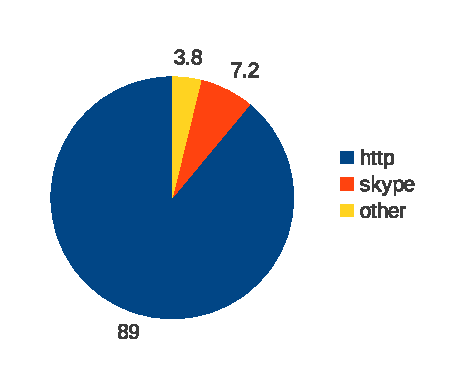
\includegraphics[width=6cm]{images/application_fact_port_80.eps}
	\caption{Application traffic running on TCP port 80 \citep{SchatzmanThesis2012}} 
	\label{fig:tcp_port80}
\end{figure}

However, by performing deep packet inspection \citet{SchatzmanThesis2012} has shown that the heuristic port based traffic preselection is not ideal, since a handful other applications are running on \gls{TCP}  port 80, presumably for firewall avoidance purposes. As shown in figure \ref{fig:tcp_port80}, the most relevant application running on \gls{TCP} port 80 -- besides \gls{HTTP} -- is Skype with a share of $7.2\%$ of all \gls{TCP} port 80 traffic. 

This \gls{TCP} port 80 based Skype traffic yields a completely different reachability characteristic. As shown by \citet{SchatzmanThesis2012}, there is a significantly higher amount of Skype \gls{TCP} port 80 sockets not reachable compared to \emph{normal} web server sockets of \gls{cdn} which is illustrated by figure \ref{fig:skype_traffic}. This exacerbates the reliable detection of network outages. 

\begin{figure}
	[ht] \centering
	\includegraphics[width=12cm]{images/application_fact.eps}
	\caption{Unreachable TCP port 80 sockets differentiated by Skype and CDN application running on these sockets. \citep{SchatzmanThesis2012}} 
	\label{fig:skype_traffic}
\end{figure}

To this end, this thesis proposes a new type of traffic preselection which includes only traffic towards stable and reliable services. This is achieved by selecting traffic based on the past stability and popularity characteristics of remote services instead of the current heuristic port-based traffic preselection.

In detail, remote services are monitored and analyzed on longer time scales so that the deduced statistical information allows the characterization of the services. Consequently, only traffic towards sockets which are characterized as stable are monitored by \gls{FACT}. For example, a remote web server used only by few users that is often unreachable, e.g.,due to testing or resource scarcity, should not be monitored by \gls{FACT}. In contrast, a popular content distribution host that was always reachable in the past is more relevant. 

To sum up, the overall goal of this thesis is to extend \gls{FACT} with a service monitoring and classification functionality to enhance the current rudimentary traffic preselection. In fact, this functionality should allow \gls{FACT} to focus even better on relevant connectivity issues which are related to stable and popular services.


\section{Related Work 
\label{sec:related_work}}
Due to the special interest of research and industrial vendors in the problem, there is a great effort done in the past. 
Generally, the related work with impact on this thesis can be separated into two thematically different topics.
On the one hand, there is a lot of research done in the area of reachability tracking. 
On the other hand, the topic of detecting network services is not only of interest for research and industry, but also for cyber criminals. 
In the following, both areas are briefly covered. 

\subsection{Reachability Tracking}

% Connection Tracking (Active & Passive)
Severe disruptions of the Internet's end-to-end connectivity is not a new phenomenon, there have been connectivity outages since its beginning as research project. 
Despite that the end-to-end connectivity is a very basic service of the Internet, the Internet community has not a deeply founded understanding of the problems that causes its disruption \citep{Bush:Optometry}.
A dominant share of researchers focussed on "pathological behavior related to the address space, e.g., bogon advertisements \citep{Feamster:2005}, prefix hijacking \citep{Zhang:2010}, \gls{bgp} misconfigurations \citep{Mahajan:2002} or \gls{DDoS} attacks \citep{Chen:2001}"\citep{Bush:Optometry}.

Basically, reachability can be viewed from two perspectives: \gls{data-plane} and \gls{control-plane} measurements. \citep{Feamster:2005,Zhang:2010,Mahajan:2002,Chen:2001} are mainly based on \gls{control-plane} information as publicly available BGP data for deducing knowledge about reachability. 
\citet{Bush:Optometry} pointed out that tracking \gls{data-plane} reachability with \gls{control-plane} information is heavily inaccurate due to the effect of secret peering policies, e.g., default routing. 
These allow packets to reach their destination even when a route failed to propagate through the \gls{bgp} system. 
\citet{Bush:Optometry} stated that even very basic \gls{data-plane} measurements
produce better views on reachability than \gls{bgp} observations. 
However, \gls{control-plane} based measurements are not limited to \gls{bgp} data, \citet{Markopoulou:2008} classified failures in a IP backbone network with \gls{is-is} information and tried to characterize these failures by layers as router, optical/link and maintenance. 
To sum up, \gls{control-plane} measurements of reachability are indirect and thus of limited practical usage for systematical reachability tracking approaches.

In contrast, measurements of the \gls{data-plane} are direct and can be more accurate regarding end-to-end connectivity. 
\Gls{data-plane} measurements can be divided into active probes and passive monitoring. 
Whereas active probes generates additional traffic towards the observed address space of the Internet, passive monitoring relies mainly on the traffic of servers and clients of the network or the traffic towards them. 

Active probing is widely used for end-to-end reachability problem detection, ranging from rudimentary debugging tools as ping \citep{PING}, paris traceroute \citep{traceroute} or nmap \citep{Nmap} to highly sophisticated, automated
outage detection tools as Hubble \citep{Katz:2008} or PlanetSeer \citep{Zhang:2004}. 
\citet{Bush:Optometry} pointed out that there exist some important limitations of active probing approaches as filtered packets by firewall and \gls{nat} devices or suboptimal routing which result in intermittent problems as packet rerouting.
Furthermore, there is no active probing technique known which is able to record the return-path in addition to the forward-path which can be extracted for example with traceroute probes. 
It is not generally true to deduce that forward-path reachability implies return-path reachability as well, since there may be intermittent problems caused for example by suboptimal routing \citep{Bush:Optometry}.

% Pingin' in the rain (Schulman/Spring)
\citet{Quan12a} implemented an Internet outage detection engine which is able to actively probe a representative part of the Internet and correlate outage events with \gls{control-plane} information. 
This is achieved by a sophisticated target selection approach. 
However, this approach is avoiding some of the drawbacks of active probing as blockage by firewalls and \gls{nat} devices by clearly state that they are able to track the "analyzable" \gls{IPv4} address space of the Internet which represents the space which is answering on their active probes.
The future scalability of this approach -- especially with respect to \gls{IPv6} -- is questionable. 

%_--- PASSIVE --
Besides the big amount of different approaches using active probing, only few approaches are using passive monitoring for reachability tracking. 
\citet{Dainotti:2011:ACI} presented an approach for an in-depth analysis of connectivity outages caused by political censorship by combining observations from \gls{bgp} data, \gls{data-plane} information as backscatter measurements of the UCSD network telescope, and active probing measurements from the Archipelago Measurement Infrastructure. 
Remarkable is their approach of (passively) monitoring of the unsolicited \gls{data-plane} traffic that shed light on Libya's attempts on deploying packet filters for enforcing the Internet censorship. 
They concluded that this unsolicited and unwanted traffic captured by network telescopes may "illuminate many different types of macroscopic events, including but not limited to broad-scale packet-filtering-based censorship, which is not observable by \gls{bgp} data."\citep{Dainotti:2011:ACI}.

% evtl iatmon noch..
%\citet{SchatzmannPAM2011} aim to detect reachability problem by passively monitoring \gls{data-plane} measurement and aggregate unresponsive connection attempts on network- and AS-level.
\subsection{Service Detection} 

% Service Detection (Active & Passive, completeness vs. scalability / importance)
The discovery and characterization of services in the Internet is most successfully done on a massive scale, ironically not by researchers but by worms and other malware\citep{Chen:2007}. 
Generally, service detection methods can mainly be grouped into two approaches: passive monitoring and active probing. 
As \citet{Bartlett07b} pointed out, active probing is able to detect all visible and scannable services, which is thus invasive and legally constrained. 
On the other hand, passive monitoring is able to find transient services, but fails to detect idle services. 
In their work, they compared the "accuracy of passive and active approaches to service discovery and showed that they are complimentary"\citep{Bartlett07b}. 
They concluded that best results are achieved by combining a long lasting passive monitoring with multiple active scans, thus forming a hybrid approach\citep{Bartlett07b}. 

\citet{Leonard:2010} developed an Internet-wide service scanner called IRLscanner. 
They designed their scanner to maximize politeness to remote networks by smartly choosing adequate scanning rates. 

% Webster active / passive
\section{Contribution 
\label{sec:contribution}}
This master thesis contributions are the following: 
\begin{itemize}
	\item qualitative analysis of remote server sockets found by a passive approach based on \citet{Schatzmann:Mining,Schatzmann:Dissection, Schatzmann:Tracing} regarding their characteristics of stability, visibility and popularity.
	\item synthesis of the findings of this characterization for enhancing the traffic selection for tracking remote connectivity issues based on the approach of \citet{SchatzmannPAM2011}.
\end{itemize}

\section{Outline
\label{sec:outline}}



\todo{Write me at last..}



%%!TEX root = ./main.tex
\chapter{Background\label{Problem}}


% Implementation


%!TEX root = ./main.tex
\chapter{Approach
\label{chapter:approach}}

\section{Methodology
\label{section:methodology}}

To achieve this goal of enhancing the reporting functionalities of FACT with
knowledge about the past stability and popularity characteristics, the following
three steps are planned for extending FACT as illustrated in figure
\ref{fig:FACT}.
\begin{figure}
	[ht] \centering
	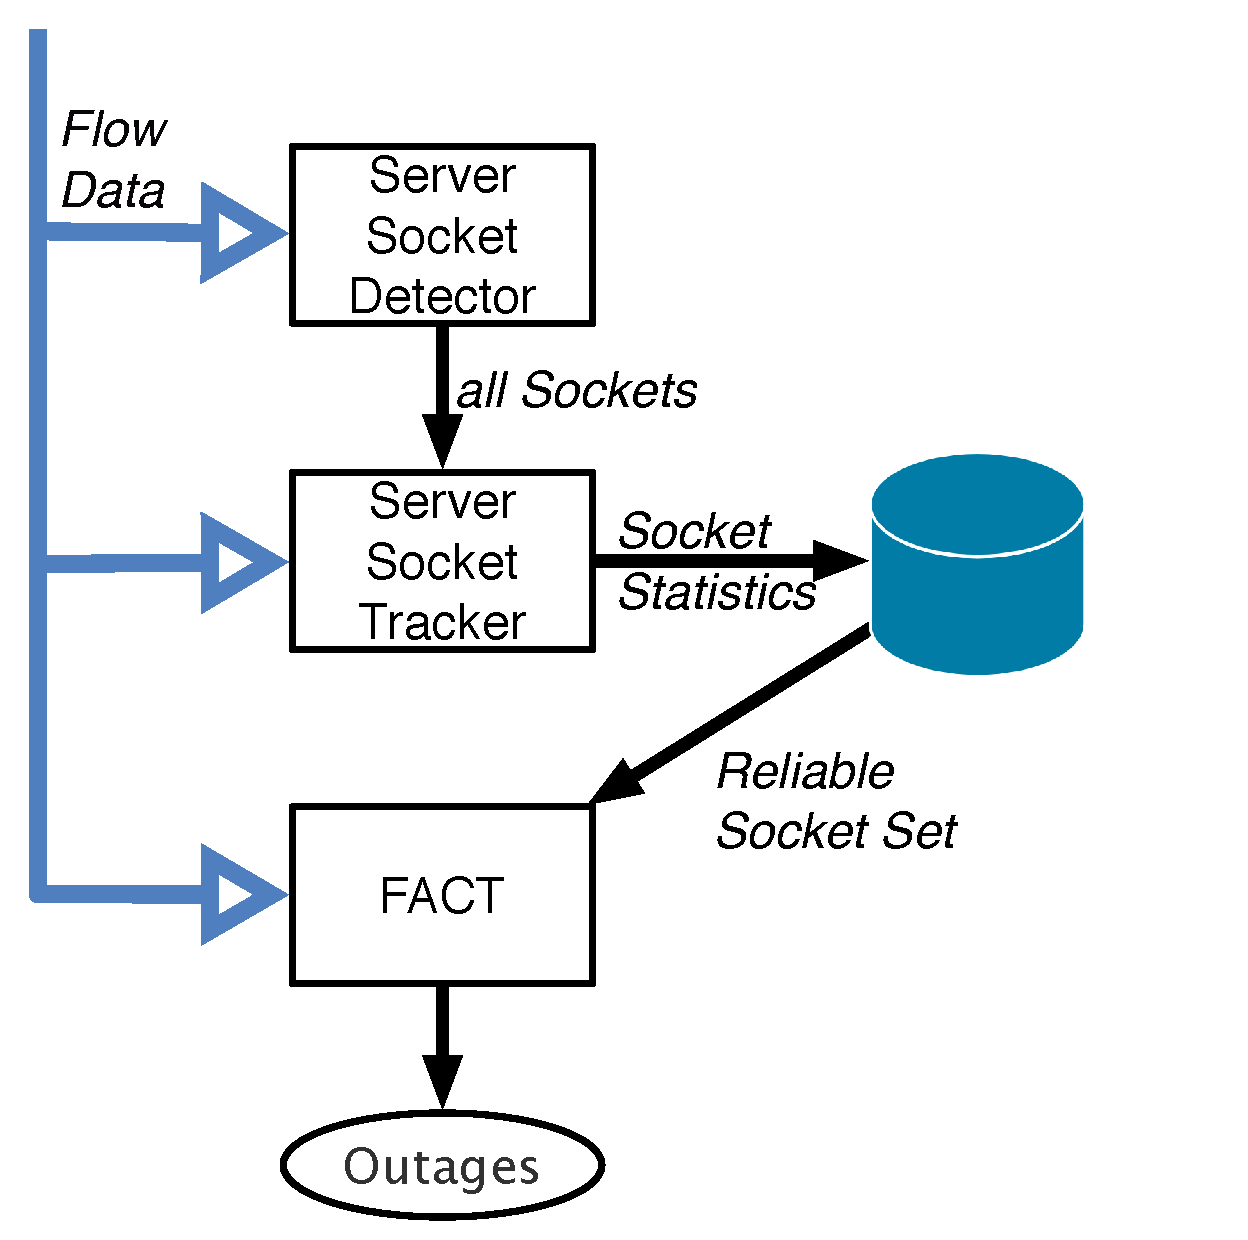
\includegraphics[width=8.5cm]{images/Approach_blockdiagram.eps}
	\caption{Interactions of new components with FACT} 
	\label{fig:FACT} 
\end{figure}

In a first step, a server socket detector is implemented. The challenge of the
server socket detection lies in the fact that the netflow data does not provide
enough precise timing information to determine which flow is originated from the
client and thus determine the server's socket. Therefore, the server socket
detection is achieved by the assumption that server sockets act as concentrators
in the sense that several clients have connections to the identical server
socket and bases on the work shown in
\cite{Schatzmann:Dissection,Schatzmann:Mining,Schatzmann:Tracing} and is
discussed in more detail in section \ref{section:socket_detection}.

Secondly, the previously detected server sockets are continually monitored and
especially the successful and unsuccessful connection attempts are recorded by
the server socket tracker.
Furthermore, these information are used to update the statistical information of
visibility, popularity and stability. Section \ref{section:socket_tracking}
covers this step in detail.

In a third step, the number of server sockets have to be reduced and selected
such that FACT is able to use these sockets for outage tracking. In particular,
the server sockets coverage of the Internet address space has to be optimized.
It makes no sense to select only the most popular sockets if they are all
located in the same /24 network.

Finally, FACT has to be adopted to optimally use the preselected and rated
server sockets for prioritizing relevant connectivity issues by reducing outage
alerts based on single host outages of unstable services.

%%%%%%%%%%%%%%%%%%%%%%%%%%%%%%%%%%%%%%%%%%%%%%%%%%%%%%%%%%%%%%%%%%%%%%%%%%%%%%%%
\section{Data
\label{section:data}}

% briefly describe the Switch network and its topology..
% traffic volume and netflow data unsampled!
% see tech report 338 for numbers and layout?! evtl actual numbers (2012)
%%%%%%%%%%%%%%%%%%%%%%%%%%%%%%%%%%%%%%%%%%%%%%%%%%%%%%%%%%%%%%%%%%%%%%%%%%%%%%%%
\section{Flowbox
\label{section:flowbox}}

\subsection{Preprocessing}

% configured with internal prefixes, responsible for tagging flows with direction. Setting transit and internal network traffic (in-in) as invalid (filtering away)
\subsection{Connection Cache} This module is responsible for generating
bidirectional flows from the incoming unidirectional flows. This is done by
storing the flows in hash table with a hash key which is identical for incoming
and outgoing flows. For correct operation of the biflow cache, a properly
configured InOutFilter is required in front of the biflow cache since it
requires that all flows must be tagged either as outgoing or as incoming. 

\subsection{Noise Cancellation} 
\subsubsection{Fan-Out Filter}

% scanning detection and elimination
% state algorithm.. analog to tech report
\subsubsection{Noise Filter}

% remove single packet flows / unidirectional biflows...
\subsection{Detection of Server Sockets} 
\subsubsection{Server Socket Detector}

\subsubsection{Server Socket Registry}

\subsection{Monitoring of Server Sockets} 
\subsubsection{Server Socket Stability
Tracker} 
\subsubsection{Server Socket Selector}

\subsection{Connectivity Issue Detection}


%

%!TEX root = ./main.tex
%** Results.tex: What were the results achieved including an evaluation
\chapter{Evaluation\label{chapter:results}}

In order to evaluate the effect of server socket based traffic preselection, three known events were analyzed with the old port-based heuristic of FACT as well as with the new server socket based approach. Then, both results are compared and the effect of the traffic preselection on the noise of the results is qualitatively discussed.

Table \ref{table:ses_set_coverage} shows the coverage of each set with respect to their IP space coverage in absolute and relative terms. 

% state the sets which are what coverage in terms of /24, IP SPACE v4/v6
\todo{FIXME!!}
\begin{table}
	[ht] \centering 
	\begin{tabular}
		{|l|c|r|r|r|r|} \hline \multirow{2}{*}{\textbf{Socket Set}} & \multirow{2}{*}{\textbf{Number of Sockets}} & \multicolumn{2}{|c|}{\textbf{IPv4 Space}} & \multicolumn{2}{|c|}{\textbf{IPv6 Space}} \\
		\cline{3-6} & & absolute & relative & absolute & relative \\
		\hline \hline All Server Sockets & 2129033 & 694627 & 100\% & 1231 & 100\% \\
		\hline Port 80 & 610273 & 158765 & 22.85\% & 296 & 24.05\% \\
		\hline Port 53 \& 80 & 939345 & 238032 & 34.27\% & 1153 & 93.66\% \\
		\hline Port 53 \& 80 \& 443 & 1010966 & 251044 & 36.14\% & 1157 & 93.99\% \\
		\hline 
	\end{tabular}
	\label{table:ses_set_coverage}
	\caption{Coverage of server socket sets} 
\end{table}

\todo{state that socket sets are from november 2010, events are before! due to lack of time to do detection for each event }


%%%%%%%%%%%%%%%%%%%%%%%%%%%%%%%%%%%%%%%%%%%%%%%%%%%%%%%%%%%%%%%%%%%%%%%%%%%%%%%%
% EVENT 1: AMS-IX PARTITIONING
%%%%%%%%%%%%%%%%%%%%%%%%%%%%%%%%%%%%%%%%%%%%%%%%%%%%%%%%%%%%%%%%%%%%%%%%%%%%%%%%
\section{Event 1: Partitioned Internet Exchange Point}

The IXP \citet{AMS-IX}(AMS-IX) performed on March 23, 2010 a scheduled maintenance. When its connection to \citet{switch} came back, there was only a partial connectivity through this IXP, since some next-hops learned via their route servers were not properly reachable, thus traffic towards these networks are black-holed.\citep{SchatzmannPAM2011}

In consequence, several internal clients of the \citet{switch} network were complaining about unreachable external services on the next morning. Using classical debugging tools, it took more than four hours for fixing the problem by resetting a port.\citep{SchatzmannPAM2011}

\subsection{Heuristic Approach}
This event is well visible by the classical FACT, since there are quite a large number of affected users thus favoring the user aggregation approach of detecting relevant events. Figure \ref{fig:AMS_IX_FACT_REF} shows the number of unreachable BGP prefixes over time separated by the number of affected internal clients. As previously outlined the user aggregation approach tries to prioritize severe events by determining the number of affected internal users. Hence, the severity of the events is indicated by the color of the unreachable prefixes in figure \ref{fig:AMS_IX_FACT_REF}. To be precise, the pink prefixes denotes the unreachable prefixes by at least 10 distinct internal clients, the blue respectively 5 distinct internal clients.

This specific IXP partitioning event is clearly visible in figure  \ref{fig:AMS_IX_FACT_REF} from 05.00 UTC to 08:15 UTC with almost 20 unreachable BGP prefixes affecting more than 10 internal clients and almost 200 unreachable BGP prefixes in total. However, as discussed in chapter \ref{Introduction}, those unreachable prefixes affecting only 1 client are not reliable observations, thus of limited interest representing a kind of observation noise of FACT.

\begin{figure}
	[p] \centering 
	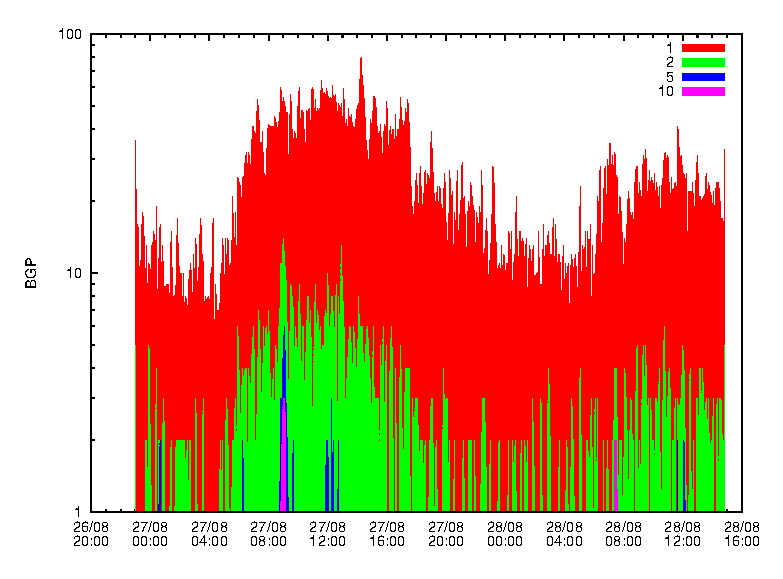
\includegraphics[width=0.75\linewidth]{images/events/2010_03_25/bgp_log_port80_ref.eps}
	\caption{Event 1: Unreachable BGP prefixes detected by the classical FACT traffic preselection based on the port-based heuristic.} 
	\label{fig:AMS_IX_FACT_REF} 
\end{figure}

\subsection{Server Socket Approach}
For evaluating the server socket bases approach, several different server socket sets are choosen, since this socket set selection process is an optimization problem as outlined in chapter \ref{chapter:integration}.

Firstly, a FACT is operated with a server socket set denoted as \emph{AllPort80SeS}, including all detected server socket listening on port 80. This socket set can directly be compared to the old heuristic approach, since it monitors a majority of those traffic as well. 

As figure \ref{fig:AMS_IX_FACT_allSES80} shows, the real event lasting from 05.00 UTC to 08:15 UTC is clearly visible equally well as in the heuristic approach from figure \ref{fig:AMS_IX_FACT_REF}. However, the server socket based approach reduces the red part indicating the number of unreachable prefixes affecting only a single internal user by at least an order of magnitude. Hence,  the event is now clearly standing out of the \emph{background event detection noise}.

Despite that fact, that the \emph{AllPort80SeS} set is not optimized at all, it outperformed the traditional approach in terms of noise reduction without significantly worsen the real event detection. This confirms the assumption that a high number of unreachable prefixes affecting only a single internal user is caused by malware and p2p churn.


\begin{figure}
	[p] \centering 
	\includegraphics[width=0.75\linewidth]{images/events/2010_03_25/bgp_log_allPort80SES.eps}
	\caption{Event 1: Unreachable BGP prefixes detected by the modified FACT traffic preselection based on all port 80 server sockets.} 
	\label{fig:AMS_IX_FACT_allSES80} 
\end{figure}


\begin{figure}
	[p] \centering 
	\includegraphics[width=0.75\linewidth]{images/events/2010_03_25/bgp_log_port80_Set_stab_0_vts_2.eps}
	\caption{Event 1: Unreachable BGP prefixes detected by the modified FACT traffic preselection based on all port 80 server sockets with visibility of at least 2 days.} 
	\label{fig:AMS_IX_FACT_allSES80VTS2} 
\end{figure}

\begin{figure}
	[p] \centering 
	\includegraphics[width=0.75\linewidth]{images/events/2010_03_25/bgp_log_port80_Set_stab_9_vts_2.eps}
	\caption{Event 1: Unreachable BGP prefixes detected by the modified FACT traffic preselection based on all port 80 server sockets with visibility of at least 2 days and stability ratio of at least $90\%$.} 
	\label{fig:AMS_IX_FACT_allSES80VTS2STAB9} 
\end{figure}

\begin{figure}
	[p] \centering 
	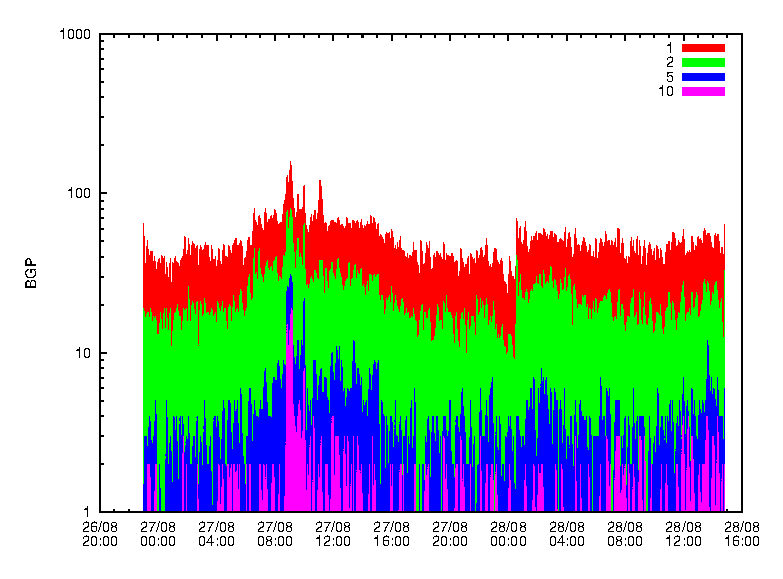
\includegraphics[width=0.75\linewidth]{images/events/2010_03_25/bgp_log_all_external.eps}
	\caption{Event 1: Unreachable BGP prefixes detected by the modified FACT traffic preselection based on all detected server sockets} 
	\label{fig:AMS_IX_FACT_allSES} 
\end{figure}

\begin{figure}
	[p] \centering 
	\includegraphics[width=0.75\linewidth]{images/events/2010_03_25/bgp_log_Set_var_0_1_stab_9_vts_2.eps}
	\caption{Event 1: Unreachable BGP prefixes detected by the modified FACT traffic preselection based on the $70\%$ most popular server sockets limited to those with a visibility of at least 2 days and stability ratio of at least $90\%$.} 
	\label{fig:AMS_IX_FACT_popularVTS2STAB9} 
\end{figure}


%%%%%%%%%%%%%%%%%%%%%%%%%%%%%%%%%%%%%%%%%%%%%%%%%%%%%%%%%%%%%%%%%%%%%%%%%%%%%%%%
% EVENT 2: TIER-1 BLACK-HOLING
%%%%%%%%%%%%%%%%%%%%%%%%%%%%%%%%%%%%%%%%%%%%%%%%%%%%%%%%%%%%%%%%%%%%%%%%%%%%%%%%
\newpage
\section{Event 2: Reverse path traffic black-holing}

On May 18, 2010, the operators of the SWITCH network were assigned to investigate an reported issue that all services in an external /24 network were not accessible from the SWITCH network between 08:30 and 08:45 UTC. According to SWITCH, the problem was most likely due to an issue of an tier-1 provider which black-holed parts of the reverse traffic towards the SWITCH network\citep{SchatzmannPAM2011}.

Unfortunately, the operators were neither able to tell how many internal users were affected nor how many external networks were unreachable during this period of time. However with the help of FACT, this issue can be further assessed with respect to the severity of the event\citep{SchatzmannPAM2011}.

\subsection{Heuristic Approach}

\begin{figure}
	[p] \centering 
	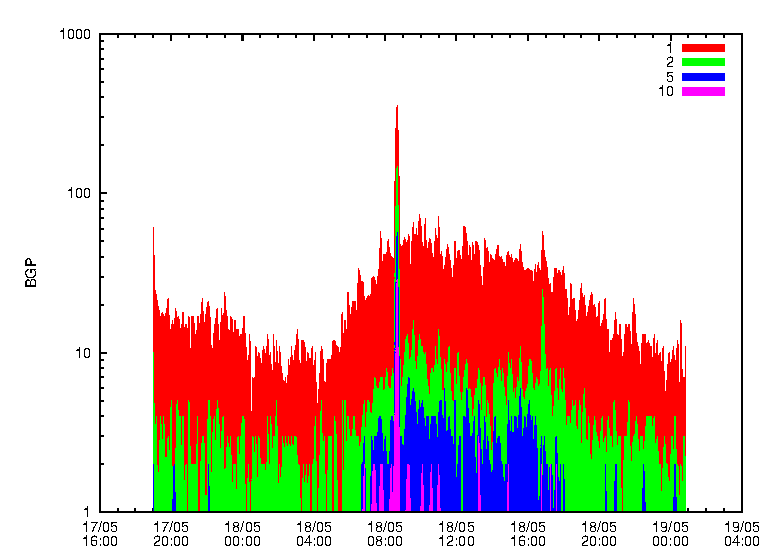
\includegraphics[width=0.75\linewidth]{images/events/2010_05_18/bgp_log_port80_ref.eps}
	\caption{Event 2: Unreachable BGP prefixes detected by the classical FACT traffic preselection based on the port-based heuristic.} 
	\label{fig:TIER1_FACT_REF} 
\end{figure}

\subsection{Server Socket Approach}

\begin{figure}
	[p] \centering 
	\includegraphics[width=0.75\linewidth]{images/events/2010_05_18/bgp_log_allPort80SES.eps}
	\caption{Event 2: Unreachable BGP prefixes detected by the modified FACT traffic preselection based on all port 80 server sockets.} 
	\label{fig:TIER1_FACT_allSES80} 
\end{figure}


\begin{figure}
	[p] \centering 
	\includegraphics[width=0.75\linewidth]{images/events/2010_05_18/bgp_log_port80_Set_stab_0_vts_2.eps}
	\caption{Event 2: Unreachable BGP prefixes detected by the modified FACT traffic preselection based on all port 80 server sockets with visibility of at least 2 days.} 
	\label{fig:TIER1_FACT_allSES80VTS2} 
\end{figure}

\begin{figure}
	[p] \centering 
	\includegraphics[width=0.75\linewidth]{images/events/2010_05_18/bgp_log_port80_Set_stab_9_vts_2.eps}
	\caption{Event 2: Unreachable BGP prefixes detected by the modified FACT traffic preselection based on all port 80 server sockets with visibility of at least 2 days and stability ratio of at least $90\%$.} 
	\label{fig:TIER1_FACT_allSES80VTS2STAB9} 
\end{figure}

\begin{figure}
	[ht] \centering 
	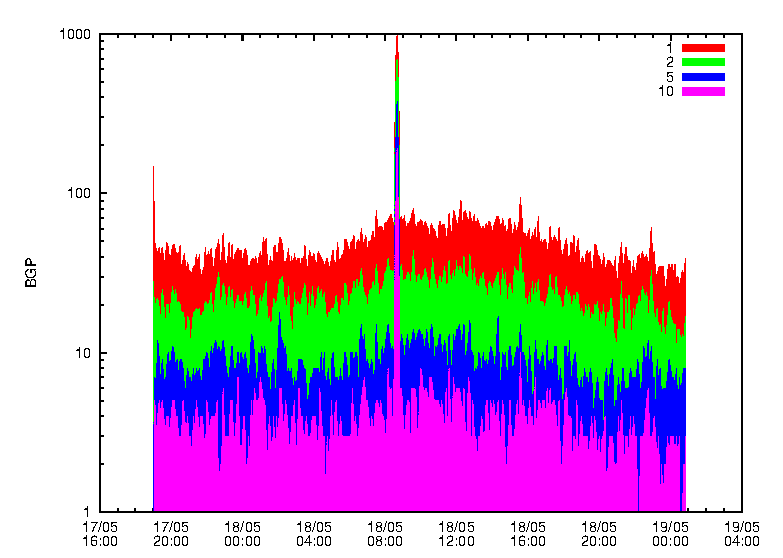
\includegraphics[width=0.75\linewidth]{images/events/2010_05_18/bgp_log_all_external.eps}
	\caption{Event 2: Unreachable BGP prefixes detected by the modified FACT traffic preselection based on all detected server sockets} 
	\label{fig:TIER1_FACT_allSES} 
\end{figure}


\begin{figure}
	[ht] \centering 
	\includegraphics[width=0.75\linewidth]{images/events/2010_05_18/bgp_log_Set_var_0_1_stab_9_vts_2.eps}
	\caption{Event 2: Unreachable BGP prefixes detected by the modified FACT traffic preselection based on the $70\%$ most popular server sockets limited to those with a visibility of at least 2 days and stability ratio of at least $90\%$.} 
	\label{fig:TIER1_FACT_popularVTS2STAB9} 
\end{figure}

%%%%%%%%%%%%%%%%%%%%%%%%%%%%%%%%%%%%%%%%%%%%%%%%%%%%%%%%%%%%%%%%%%%%%%%%%%%%%%%%
% EVENT 3: RIPE / DUKE BGP EXPERIMENT
%%%%%%%%%%%%%%%%%%%%%%%%%%%%%%%%%%%%%%%%%%%%%%%%%%%%%%%%%%%%%%%%%%%%%%%%%%%%%%%%
\newpage
\section{Event 3: RIPE / DUKE BGP Experiments}

An experiment with new BGP attributes jointly performed by RIPE and the Duke 
University on August 27, 2010, resulted in several unreachable prefixes\citep{SchatzmannPAM2011}. These 
new kind of attributes has never been announced on the Internet before,  
although it was in accordance with the BGP specification\citep{ripe_duke}.

These new kind of attributes uncovered and triggered a bug in some Cisco BGP 
Routers known as the \emph{Cisco IOS XR Software Border Gateway Protocol Vulnerability (SA-20100827-BGP)}\citep{cisco_vulnerability}. In particular, the announcements with the new attributes were corrupted 
by the Cisco Routers and send to their peers. Consequently, their peers detected 
the corruption and dropped the entire peering session\citep{ripe_duke}.

\subsection{Heuristic Approach}

\subsection{Server Socket Approach}


%%!TEX root = ./main.tex
\chapter{Conclusion\label{Conclusion}}

\section{Conclusion}



\section{Future Work}
% characterize ses by time based activity (night / day, working week, weekend etc.)

% smarter socket set selection => density of network by choosing only the popularst sockets of each network

% automatization of process => danger of excluding sockets affected by events
% => consider full last week?  

% general optimization problem solving approach as simulated annealing => limit number of sockets => pareto front of sockets

% consider different selection methods as clustering analysis approaches, e.g. k-means etc => distance function include also network considerations.. etc. 

% near future public release of FlowBox and FACT


% Appendix-mode in Latex
\appendix

% Set enumeration to alphabetical  characters.
\renewcommand{\thepart}{\Alph{part}}

%%!TEX root = ./main.tex

\chapter{Appendix}
\label{appendix}
\section{Prefix Files for FACT}

Switchextract is a neat little perl script for generating the required prefix files for the FilterInOut and the Analyser of FACT. It may be found in the tool folder of the FACT sourcecode. For correctly using these perl script, the following preliminary work have to be done:
\begin{enumerate}
	\item Download and install bgpdump from the RIPE RIS project.
	\item Download the bgpdump file of the desired date from a suitable route collector - the best from the default free rrc00.ripe.net.
	\item Adjust your own AS number within the perl script switchextract.pl, i.e. replace 559 at line 24 with your own AS number.
\end{enumerate}

Then the following steps must be executed:
\begin{enumerate}
	\item Create a file bgpdump.txt with bgpdump: \newline\texttt{bgpdump bview.XXXXXX.XXXX.gz -m > bgpdump.txt}
	\item Call the perl script switchextract.pl: \newline\texttt{perl switchextract.pl bgpdump.txt prefixes.txt}
	\item prefixes.txt has to be moved or linked to the analyser configuration folder of FACT
	\item switch\_prefixes.txt is needed by the FilterInOut and has to be moved or linked to the configuration folder of FilterInOut.
\end{enumerate}



%** Originalproblem.tex: The problem statement you received.
%
%%!TEX root = ./main.tex

\section{Orginal Problem}

\includegraphics[width=\textwidth, page=1]{ThesisDescription.pdf}
\newpage
\includegraphics[width=\textwidth, page=2]{ThesisDescription.pdf}
\newpage
\includegraphics[width=\textwidth, page=3]{ThesisDescription.pdf}

%\listoffigures
%!TEX root = ./main.tex
\bibliographystyle{apalike} 
\bibliography{95_bib}

%

%!TEX root = ./main.tex
\chapter*{Eigenständigkeitserklärung} Ich erkläre hiermit, dass es sich bei
der von mir eingereichten schriftlichen Arbeit mit dem Titel
\textbf{"Who turned off the Internet? Mining Temporary Unreachability"} um eine von mir selbständig und in eigenen Worten verfasste
Originalarbeit handelt.\\

\vspace{5mm} \textbf{Verfasser:}\\
Daniel Aschwanden\\

\vspace{5mm} \textbf{Betreuer:}\\
Dominik Schatzmann\\
Dr. Bernhard Ager\\

\vspace{5mm} Mit meiner Unterschrift bestätige ich, dass ich über fachübliche
Zitierregeln unterrichtet worden bin und das Merkblatt
(\url{http://www.ethz.ch/students/exams/plagiarism_s_de.pdf}) gelesen und
verstanden habe. Die im betroffenen Fachgebiet üblichen Zitiervorschriften sind
eingehalten worden.
Eine Überprüfung der Arbeit auf Plagiate mithilfe elektronischer Hilfsmittel
darf vorgenommen werden.\\

\vspace{15mm} 
\begin{tabular}
	{l p{0.3
	\textwidth} r} Zürich, 17.10.2012 &&
	Daniel Aschwanden \\
\end{tabular}

\vfil
%!TEX root = ./main.tex

%%%%%%%%%%%%%%%%%%%%%%%%%%%%%%%%%%%%%%%%%%%%%%%%%%%%%%%%%%%%%%%%%%%%%%%%%%%%%%%%
% GLOSSAR
%%%%%%%%%%%%%%%%%%%%%%%%%%%%%%%%%%%%%%%%%%%%%%%%%%%%%%%%%%%%%%%%%%%%%%%%%%%%%%%%
% control-plane
\newglossaryentry{control-plane}{
	name=control-plane,
	description={}
}

% data-plane
\newglossaryentry{data-plane}{
	name=data-plane,
	description={}
}


\newglossaryentry{osi-mod}{
	name=Open Systems Interconnection Reference Model,
	description={describes the layered architecture of the Internet, standardized by ISO/IEC 7498-1}
}

% NetFlow
\newglossaryentry{netflow}{
	name=NetFlow,
	description={is a network protocol for collecting IP traffic information and was originally developed by Cisco Systems}
}

\newglossaryentry{server socket}{
	name={server socket},
	description={is a socket with a process listening to incoming connections and thus offering a network service.}
	plural={server sockets},
}


%%%%%%%%%%%%%%%%%%%%%%%%%%%%%%%%%%%%%%%%%%%%%%%%%%%%%%%%%%%%%%%%%%%%%%%%%%%%%%%%
% ACRONYMS
%%%%%%%%%%%%%%%%%%%%%%%%%%%%%%%%%%%%%%%%%%%%%%%%%%%%%%%%%%%%%%%%%%%%%%%%%%%%%%%%
% OSI
\newacronym{osi}{OSI}{\Gls{osi-mod}}

% ISP
\newacronym{isp}{ISP}{Internet service provider}

% BGP
\newacronym{bgp}{BGP}{Border Gateway Protocol}
% AS
\newacronym{AS}{AS}{autonomous system}

% SLA
\newacronym{sla}{SLA}{service level agreement}

% IS-IS
\newacronym{is-is}{IS-IS}{Intermediate System to Intermediate System Protocol}

% FACT
\newacronym{FACT}{FACT}{Flow-based Approach for Connectivity Tracking}

% NAT
\newacronym{nat}{NAT}{network address translation}

% CDN
\newacronym{cdn}{CDN}{content distribution networks}

% TCP
\newacronym{TCP}{TCP}{Transmission Control Protocol}

% UDP
\newacronym{UDP}{UDP}{User Datagram Protocol}

% IP
\newacronym{IPv4}{IPv4}{Internet Protocol version 4}
\newacronym{IPv6}{IPv6}{Internet Protocol version 6}

% HTTP, FTP, SSH
\newacronym{HTTP}{HTTP}{Hypertext Transfer Protocol}
\newacronym{FTP}{FTP}{File Transfer Protocol}
\newacronym{SSH}{SSH}{Secure Shell}
\newacronym{NTP}{NTP}{Network Time Protocol}

% P2P
\newacronym{p2p}{P2P}{peer-to-peer}

% DDoS
\newacronym{DDoS}{DDoS}{distributed denial of service}

% SES
\newacronym{ses}{SeS}{server socket}










\end{document}

%%% Local Variables:
%%% mode: latex
%%% TeX-master: "documentation"
%%% End:
